\begin{quote}
Methods of managing projects, including learning projects, range from
more formal and structured to casual and unstructured. As a facilitator,
you'll see your peeragogy community constantly adjust, as it seeks an
equilibrium between order and chaos, ideally allowing everyone to be
involved at their own pace without losing focus, and in such a manner
that the collective can deliver.
\end{quote}

\begin{center}
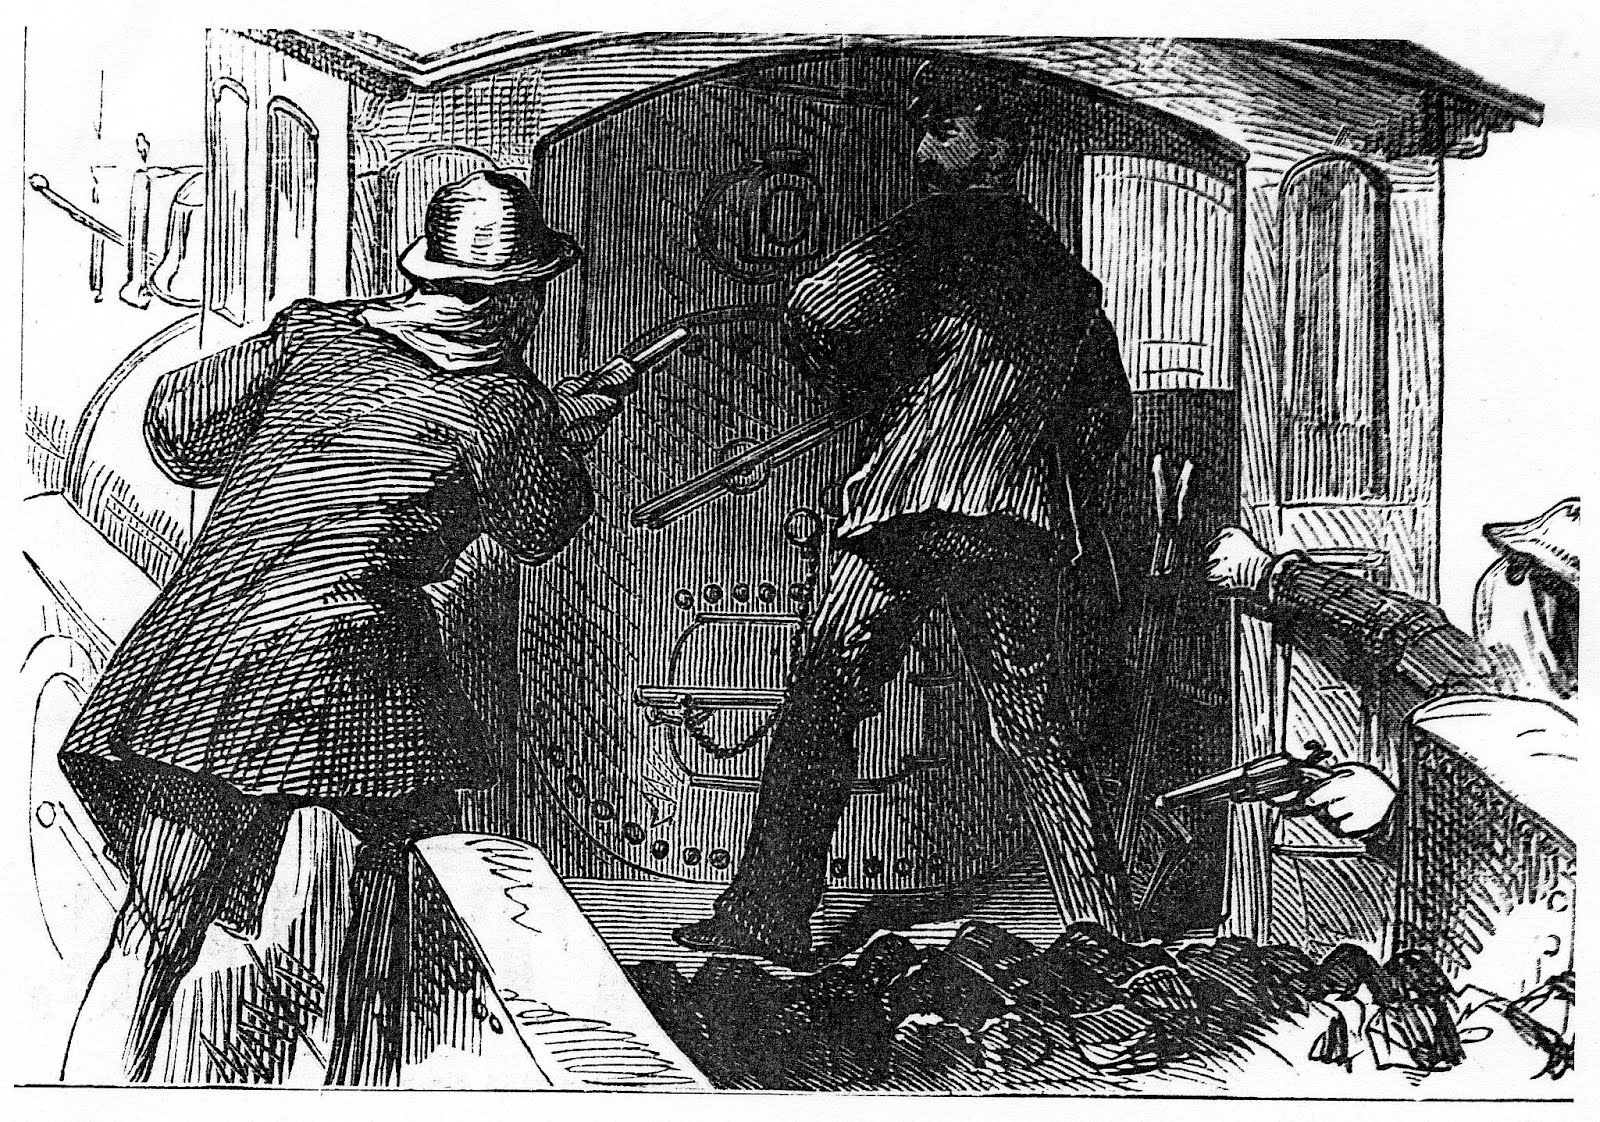
\includegraphics[width=.9\textwidth]{../pictures/james-gang.jpg} \\
Hey you, stop this train!
\end{center}

For teachers reading this, and wondering how to use peeragogy to improve
participation in their classrooms, it's really quite simple: reframe the
educational vision using peeragogical eyes. Recast the classroom as a
community of people who learn together, the teacher as facilitator, and
the curriculum as a starting point that can be used to organize and
trigger community engagement. However, just because it's simple doesn't
mean it's easy! Whatever your day job may be, consider: how well do the
various groups you participate in work together -- even when the members
ostensibly share a common purpose? Sometimes things tick along nicely,
and, presumably, sometimes it's excruciating. What's your role in all of
this? How do \emph{you} participate?



\subsection{Guidelines for participation}

\begin{itemize}
\item
  Accept that some people want to watch what is going on before jumping
  in. This doesn't mean you have to keep them hanging around forever.
  After a while, you may un-enroll people who don't add any value to the
  community. In our Peeragogy project, we've asked people to explicitly
  re-enroll several times. Most do renew; some leave.
\item
  Accept that people may only contribute a little: if this contribution
  is good it will add value to the whole.
\item
  Understand that you can not impose strict deadlines on volunteers;
  adjust targets accordingly.
\item
  Let your work be ``open'' in the sense described in Wikipedia's
  \href{http://en.wikipedia.org/wiki/Wikipedia:Neutral\_point\_of\_view}{Neutral
  Point of View} policy.
\item
  Give roles to participants and define some ``energy centers'' who will
  take the lead on specific items in the project.
\item
  Organize regular face-to-face or online meetings to talk about
  progress and what's needed in upcoming days/weeks.
\item
  Ask participants to be clear about when they will be ready to deliver
  their contributions.
\item
  Have clear deadlines, but allow contributions that come in after the
  deadline -- in general, be flexible.
\item
  Add a newcomer section on your online platform to help new arrivals
  get started. Seasoned participants are often eager to serve as
  mentors.
\end{itemize}
When we think about project management in an organization, we often
relate to well-established tools and processes. For example, we will use
the \href{http://www.pmi.org/PMBOK-Guide-and-Standards.aspx}{Project
Management Body of Knowledge} (PMBOK) as a standard. For the Project
Management Institute (PMI) and most workers, those standards are the key
to project success. In classical project management, tasks and deadlines
are clearly defined. We will, for example, use
\href{http://en.wikipedia.org/wiki/PERT}{Program Evaluation and Review
Technic} (PERT) to analyze and represent tasks. We often represent the
project schedule using a
\href{http://en.wikipedia.org/wiki/Gantt\_chart}{Gantt chart}. Those are
just two of the project management tools that illustrate how project
management rests firmly on its engineering background. In those very
structured projects, each actor is expected to work exactly as planned
and to deliver his part of the work on time; every individual delay
potentially leading to a collective delay.

Peeragogy projects often expect to break the
\href{http://en.wikipedia.org/wiki/1\%25\_rule\_\%28Internet\_culture\%29}{90/9/1
rule}, with everyone participating, not just a few. Once again, some
participants may not contribute often -- but one really good idea is
actually a major contribution. See
\href{http://peeragogy.org/practice/antipatterns/misunderstanding-power/}{Misunderstanding
Power} for some further reflections on these matters.
